\documentclass[UTF8]{ctexart}
\usepackage{amsmath}
\usepackage{amssymb}
\usepackage{background}
\usepackage{booktabs}
\usepackage{caption}
\usepackage{enumitem}
\usepackage{fancyhdr}
\usepackage{float}
\usepackage{fontspec}
\usepackage{geometry}
\usepackage[bookmarksnumbered = true, pdfborder=0 0 0]{hyperref}
\usepackage{kbordermatrix} % 会标注信息的矩阵
\usepackage{listings}
\usepackage{tasks}
\usepackage{tcolorbox}
\tcbuselibrary{breakable}
\usepackage{tikz}
\usetikzlibrary{arrows.meta, positioning, calc, shapes.geometric}
\usepackage[table]{xcolor}

\geometry{a5paper, top=0.1cm, left=1cm, right=1cm, bottom=1cm, footskip=0.1cm}
\setCJKmainfont[BoldFont={汉仪文黑-85W},ItalicFont={汉仪文黑-55W}]{汉仪文黑-55W}
\setfontfamily\Issue{Century Schoolbook}
\setfontfamily\Genshin{Genshin Teyvat Lingua Franca}
\newCJKfontfamily\TitleFont{思源宋体 CN Heavy}
\newfontfamily\timesnewroman{Times New Roman}

%————————————————可变部分——————————————————
\settasks{label={\Alph*.\ }, label-format={\color{cyan!50!black}}, item-format={\color{cyan!50!black}}}
\newcommand\col[1]{\textcolor{green!50!black}{#1}}
\newcommand\coll[1]{\textcolor{blue}{#1}}
\newcommand\dotting{\ .\ }
%\setlist[enumerate]{itemsep=0pt, parsep=0pt}
%\setlist[itemize]{itemsep=0pt, parsep=0pt}
\captionsetup{labelfont=bf, font=small}
\CTEXsetup[format = {\bfseries\large}]{subsection}

\newcommand\FIRST{\textsc{First}}
\newcommand\FOLLOW{\textsc{Follow}}
\newcommand\NULLABLE{\textsc{Nullable}}
\newcommand\FIRSTS{\textsc{First\_s}}
\newcommand\ACTION{\textsc{Action}}
\newcommand\GOTO{\textsc{Goto}}
\newcommand\D{\text{\textbullet}}
\newcommand\OR{\ |\ }
\newcommand\ERROR{\textsc{Error}}
\newcommand\deduceone{\overset{+}{\implies}} %至少一次推导
\newcommand\deduce{\overset{*}{\implies}} %任意次推导
\newcommand\VN{V_{\mathrm{N}}} %非终结符
\newcommand\VT{V_{\mathrm{T}}} %终结符
\newcommand\GEN{\mathrm{gen}}
\newcommand\KILL{\mathrm{kill}}
\newcommand\IN{\mathrm{in}}
\newcommand\OUT{\mathrm{out}}

\lstset{
    language = C,
    basicstyle=\small\ttfamily, %注意行末有逗号!
    keywordstyle=\bfseries\color{blue!70!black},
    commentstyle=\color{cyan!90!black},
    stringstyle=\color{green!40!black},
    columns=flexible,
    numbers=left,
    numberstyle=\footnotesize,
    escapechar=`,
    frame=shadowbox,
    %rulesepcolor=\color{red!20!blue!20!green!20}
    backgroundcolor=\color{cyan!5!white},
    tabsize = 4,
    breaklines = true,
    showstringspaces = false,
}
%——————————————————————————————————————————

\pagestyle{fancy}
\fancyhf{}
\cfoot{\sffamily\footnotesize{-\ \thepage\ -}}
%

\colorlet{darkcyan}{cyan!50!black}
\newcommand\Black[1]{\textcolor[gray]{0.3}{#1}}
\newcommand\Brown[1]{\textcolor[HTML]{998A4E}{#1}}
\newcommand\Emph[1]{\textcolor{cyan!80!black}{#1}}
\newcommand\Notes[1]{\textcolor{yellow!50!black}{\small #1}}
\newcommand\Example[1]{\textcolor{cyan!70!black}{\small #1}}
\colorlet{note}{yellow!70!black}


\newcommand\IssueNumber{47}
\newcommand\Date{2024-12-22}
%\newcommand\Contributer{@金光日}
\newcommand\Subject{编译原理}
%\newcommand\Source{历年考研 408 真题}


\begin{document}
\backgroundsetup{contents=\includegraphics{上半示例.png}, center, scale=1, angle=0, opacity=1}
\BgThispage
\begin{center}
%{\scriptsize\Issue \textcolor[HTML]{C8BA83}{\Genshin WEEKLY TIPS}}
\phantom{...}

{\Large\textcolor{brown!40!white}{\makebox[10cm][s]{\Genshin WEEKLY KNOWLEDGE TIPS}}}

\vspace{-2em}

{\Huge\bfseries\TitleFont \Black{知\ 识\ 小\ 料}}


\vspace{-0.1cm}
{\footnotesize \Brown{「电计 2203 班」周常规知识整理共享}}
\end{center}

\vspace{-0.5cm}


\begin{figure}[H]
\hspace{1cm}
\begin{minipage}[t]{0.3\textwidth}
\centering
    \Brown{\Genshin ISSUE}

    \vspace{-0.6cm}
    \Huge \Issue\slshape\bfseries\Black{\IssueNumber}
\end{minipage}
\hfill
\begin{minipage}[t]{0.28\textwidth}
\centering
    \Brown{日期:\Date} \\
%\vspace{-0.1cm}
%    \Brown{贡献者:\Contributer} \\
\vspace{-0.1cm}
    \Brown{学科:\Subject} \\
%\vspace{-0.1cm}
%    \Brown{来源:\Source}
\end{minipage}
\hspace{0.8cm}
\end{figure}

{\color{cyan!50!black}
\begin{center}
  本文档对编译原理课程作出简明复习。
\end{center}}

\tableofcontents

\backgroundsetup{contents=\includegraphics{空白示例.png}, center, scale=1, angle=0, opacity=1}
\BgThispage
\newpage

\section{编译、编译器}
编译器相关概念:
\begin{itemize}[itemsep=0pt,parsep=0pt,leftmargin=1.5cm]
  \item 编译器是程序。
  \item 核心功能是将\Emph{源代码}翻译为\Emph{目标代码}。
  \item 编译器的主要功能是\Emph{翻译}和\Emph{纠错},只翻译不静态计算(代码优化除外)。
  \item 包含静态与动态计算。
  \item 史上第一个编译器是 1957 年的 Fortran 编译器。
\end{itemize}

编译器与解释器的区别:
\begin{itemize}[itemsep=0pt,parsep=0pt,leftmargin=1.5cm]
    \item \Emph{编译器}:先编译,后执行,离线式,输出的是可执行程序。
    \item \Emph{解释器}:边解释,边执行,在线式,输出的是结果。
\end{itemize}

编译器结构:
\begin{figure}[htb]
    \centering
    \begin{tikzpicture}[front/.style = {circle, minimum size=0.7cm, text width=0.8cm, align=center, fill=cyan!20, draw=cyan!50, text=darkcyan},
    back/.style = {circle, minimum size=0.7cm, text width=0.8cm, align=center, fill=green!20, draw=green, text=green!50!black},
     ->, >=Stealth, node distance=1.5cm]
        \fill[fill=cyan!10, rounded corners=2mm] (-2,-1.5) rectangle (8,1.5) node[below left, cyan!40] {前端}; % 前端
        \fill[fill=green!10, rounded corners=2mm] (-2,-4.5) node[above right, green!50] {后端} rectangle (8,-1.5); % 后端
        \node[front] (n1) at (0,0) {词法分析};
        \node[front, right=of n1] (n2) {语法分析};
        \node[front, right=of n2, node distance=2cm] (n3) {语义分析};
        \node[back, below=of n3] (n4) {代码生成};
        \node[back, left=of n4] (n5) {代码优化};
        \path[darkcyan] ($(n1.north)+(0,1.5)$) edge node[left, font=\small] {字符序列} (n1);
        \path (n1) edge node[above, font=\small] {记号序列} (n2);
        \path (n2) edge node[above, font=\small] {抽象语法树} (n3);
        \path (n3) edge node[right, font=\small] {中间代码} (n4);
        \path (n4) edge node[above, font=\small] {} (n5);
        \path (n5) edge [loop left] node[left, font=\small] {反复优化} (n5);
        \path[green!50!black] (n5) edge node[left, font=\small] {目标代码} ($(n5.south)+(0,-1.5)$);
    \end{tikzpicture}
    \caption{编译器结构(总体为\textcolor{darkcyan}{高级语言}→\textcolor{green!50!black}{目标语言})}\label{fig:编译器结构}
\end{figure}

编译器举例:把加法语言 Sum 转化为栈式计算机目标语言 Stack。例如,编译表达式 \verb!1 + 2 + 3!。
\begin{enumerate}[itemsep=0pt, parsep=0pt, leftmargin=1.5cm]
  \item 词法分析、语法分析。
  \item 语法树构建:得到如下图所示的语法树,以及后序遍历表达式 \verb!1 2 + 3 +!。
  \item 代码生成:常数结点 $n$ 对应 \verb!push n!,加法结点 $+$ 对应 \verb!add!。
  \item 代码优化:常量折叠等。
\end{enumerate}
\begin{figure}[htb]

    \begin{minipage}[t]{.6\textwidth}
    \vspace{0pt}
    \centering
        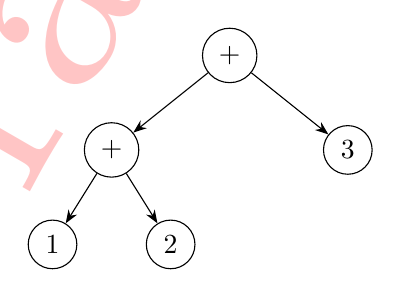
\begin{tikzpicture}[
          level 1/.style={sibling distance=30mm},
          level 2/.style={sibling distance=15mm},
          level distance=12mm,
          edge from parent/.style={->,draw},
          every node/.style={circle, draw, minimum size=1em},
          >=Stealth
        ]
        \node [circle, draw] (root) {+}
          child {node [circle, draw] (c1) {+}
            child {node [circle, draw] (c11) {1}
            }
            child {node [circle, draw] (c12) {2}
            }
          }
          child {node [circle, draw] (c2) {3}
          };
        \end{tikzpicture}
    \end{minipage}
    \begin{minipage}[t]{.39\textwidth}
    \vspace{0pt}\centering
    \begin{verbatim}
        push 1
        push 2
        add
        push 3
        add
    \end{verbatim}
    \end{minipage}
  \caption{加法语言 Sum 的示例表达式 \texttt{1 + 2 + 3} 的抽象语法树及目标代码}\label{fig:tree-1+2+3}
\end{figure}



\section{词法分析·大纲}
\subsection{词法分析的任务}
词法分析位于「前端」部分,其输出作为语法分析的输入。词法分析的任务是将\Emph{字符序列}翻译为\Emph{记号序列}。

词法分析可以手动实现,典型的例子是识别比较符号。

\begin{figure}[htb]
  \centering
  \includegraphics[width=8cm]{识别比较符号.png}
  \caption{识别比较符号}\label{fig:compare}
\end{figure}

\Notes{(注:图中的双圈为终态,星号(*)表示指针回溯。例子中的 \texttt{<>} 会被识别为不等于号,所以不是严格的 C 语法。)}

\begin{lstlisting}
token nextToken ()
    c = getChar ();
    switch (c)
        case ‘<’:
            c = getChar ();
            switch (c)
                case ‘=’: return LE;
                case ‘>’: return NE;
                default: rollback(); return LT;
        case ‘=’: return EQ;
        case ‘>’:
            c = getChar ();
            switch (c)
                case ‘=’: return GE;
                default: rollback(); return GT;
\end{lstlisting}

此外,标识符是关键字的一部分。词法分析器需要有能力判别关键字。这里可以使用\Emph{关键字哈希表},先提取标识符,然后再查表判别关键字。好的哈希表可以 $O(1)$ 地完成任务。

\subsection{正则表达式(RE)}
\Emph{正则表达式(RE)}的归纳定义:对于给定的字符集 $\varSigma$:
\begin{enumerate}[itemsep=0pt,parsep=0pt,leftmargin=1.5cm]
  \item 空串 $\varepsilon$ 是正则表达式。
  \item 任意字符集中的元素 $c\in\varSigma$ 是正则表达式。
  \item 如果 $M,N$ 是正则表达式,则它们的选择($M|N$)、连接($MN$)、闭包($M^*,N^*$)也是正则表达式。
\end{enumerate}
经过有限步运用上述规则得到的表达式是正则表达式。\Notes{(注:$\varepsilon\in M^*$。 $e$ 的闭包 $e^*$ 表示「0个或者多个$e$」)}

形式定义:$e \to \varepsilon \OR c \OR (e|e) \OR (ee) \OR e^*$

相关其他语法糖(可以在网上搜索):
\begin{itemize}[itemsep=0pt,parsep=0pt,leftmargin=1.5cm]
  \item $e+$:1 个或者多个 $e$,即 $ee^*$
  \item $e?$:0 个或者 1 个 $e$,即 $\varepsilon|e$
  \item $[c_1-c_n]$:表示 $c_1,c_2,\dots,c_n$ 的选择,即 $c_1\OR c_2\OR\dots\OR c_n$
\end{itemize}

举例:
\begin{enumerate}
  \item 识别关键字 \verb!while! 的表达式:\verb!e -> while!。
  \item 识别标识符的表达式:\verb!e -> [a-zA-Z_][a-zA-Z0-9_]*!。(开头为字母/下划线,后续为字母/数字/下划线,后续的字符可出现0次或多次。)
  \item 识别十进制自然数的表达式:\verb!e -> 0 | [1-9][0-9]*!
\end{enumerate}

\subsection{有限状态自动机(FA)}
\Emph{有限状态自动机 (FA)} 的形式定义:$M = (\varSigma, S, q_0, F, \delta) =$ (字母表,状态集,初状态,终结状态集,转移函数)。给定一个字符串,经过 FA 以后得到一个布尔返回值,表示接受/不接受。

字符串可接受,意思是\Emph{存在}一条路径可使得 DFA 停在终结状态。

\begin{itemize}
  \item 确定性有限状态自动机 (\Emph{DFA}):对任意的字符,最多有一个状态可以转移;
  \item 非确定性有限状态自动机 (\Emph{NFA}):对任意的字符,有一个或多个状态可以转移;
\end{itemize}

DFA 可以用关联矩阵实现。对于特定的状态行和字符列,给出下一个状态值作为矩阵元素。

\section{词法分析·自动生成}
\subsection{RE→NFA:Thompson算法}
\Emph{Thompson算法}递归实现,代码精简。其实就是将正则表达式的每一条规则直接转化为相应的 NFA 图。

\begin{table}[htb]
  \centering
  \begin{tabular}{rlcl}
    $e$ & $\to \varepsilon$ & 空字符 &
    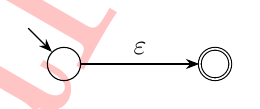
\begin{tikzpicture}[doublecircle/.style={circle,draw,double,minimum size=11pt}, state/.style={circle,draw,minimum size=12pt}, ->, >=Stealth, node distance=1.5cm]
        \node[state] (q0) {};
        \node[doublecircle, right=of q0] (q1) {};
        \path (q0) edge node[above] {$\varepsilon$} (q1);
        \draw ($(q0.north west) + (-0.3cm, 0.3cm)$) to (q0);
    \end{tikzpicture}\\

    & $\to c$ & 单字符 &
    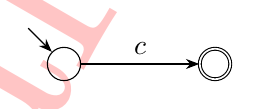
\begin{tikzpicture}[doublecircle/.style={circle,draw,double,minimum size=11pt}, state/.style={circle,draw,minimum size=12pt}, ->, >=Stealth, node distance=1.5cm]
        \node[state] (q0) {};
        \node[doublecircle, right=of q0] (q1) {};
        \path (q0) edge node[above] {$c$} (q1);
        \draw ($(q0.north west) + (-0.3cm, 0.3cm)$) to (q0);
    \end{tikzpicture}\\

    & $\to e_1e_2$ & 连接 &
    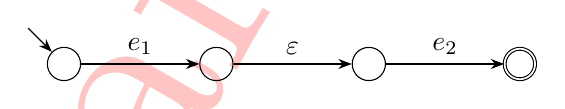
\begin{tikzpicture}[doublecircle/.style={circle,draw,double,minimum size=11pt}, state/.style={circle,draw,minimum size=12pt}, ->, >=Stealth, node distance=1.5cm]
        \node[state] (q0) {};
        \node[state, right=of q0] (q1) {};
        \node[state, right=of q1] (q2) {};
        \node[doublecircle, right=of q2] (q3) {};
        \path (q0) edge node[above] {$e_1$} (q1);
        \path (q1) edge node[above] {$\varepsilon$} (q2);
        \path (q2) edge node[above] {$e_2$} (q3);
        \draw ($(q0.north west) + (-0.3cm, 0.3cm)$) to (q0);
    \end{tikzpicture}\\

    & $\to e_1|e_2$ & 选择 &
    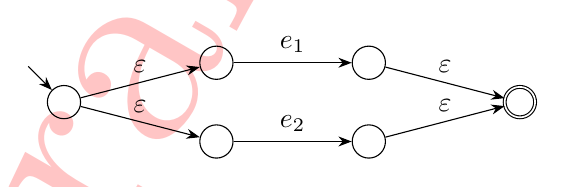
\begin{tikzpicture}[doublecircle/.style={circle,draw,double,minimum size=11pt}, state/.style={circle,draw,minimum size=12pt}, ->, >=Stealth, node distance=1.5cm]
        \node[state] (q0) {};
        \node[state, right=of q0, yshift=0.5cm] (q1) {};
        \node[state, right=of q1] (q2) {};
        \node[state, right=of q0, yshift=-0.5cm] (q3) {};
        \node[state, right=of q3] (q4) {};
        \node[doublecircle, right=of q4, yshift=0.5cm] (q5) {};

        \path (q0) edge node[above] {$\varepsilon$} (q1);
        \path (q0) edge node[above] {$\varepsilon$} (q3);
        \path (q1) edge node[above] {$e_1$} (q2);
        \path (q3) edge node[above] {$e_2$} (q4);
        \path (q2) edge node[above] {$\varepsilon$} (q5);
        \path (q4) edge node[above] {$\varepsilon$} (q5);
        \draw ($(q0.north west) + (-0.3cm, 0.3cm)$) to (q0);
    \end{tikzpicture}\\

    & $\to e^*$ & 闭包 &
    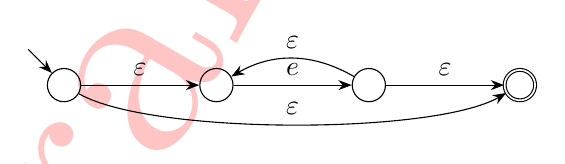
\begin{tikzpicture}[doublecircle/.style={circle,draw,double,minimum size=11pt}, state/.style={circle,draw,minimum size=12pt}, ->, >=Stealth, node distance=1.5cm]
        \node[state] (q0) {};
        \node[state, right=of q0] (q1) {};
        \node[state, right=of q1] (q2) {};
        \node[doublecircle, right=of q2] (q3) {};
        \path (q0) edge node[above] {$\varepsilon$} (q1);
        \path (q1) edge node[above] {$e$} (q2);
        \path (q2) edge node[above] {$\varepsilon$} (q3);
        \path (q0) edge [bend right, looseness=0.5] node[above] {$\varepsilon$} (q3);
        \path (q2) edge [bend right] node[above] {$\varepsilon$} (q1);
        \draw ($(q0.north west) + (-0.3cm, 0.3cm)$) to (q0);
    \end{tikzpicture}\\
  \end{tabular}
  \caption{Thompson算法构造NFA规则}\label{fig:Thompson}
\end{table}

示例:(本例贯穿整章)由正则表达式 $a(b|c)^*$ 构造的 NFA 如下图 \ref{fig:NFA-example} 所示。在图中,$n_3\sim n_8$ 对应 $b|c$,$n_2\sim n_9$ 对应 $(b|c)^*$,并与 $n_0,n_1$ 构成 $a(b|c)^*$。
\begin{figure}[htb]
    \centering
    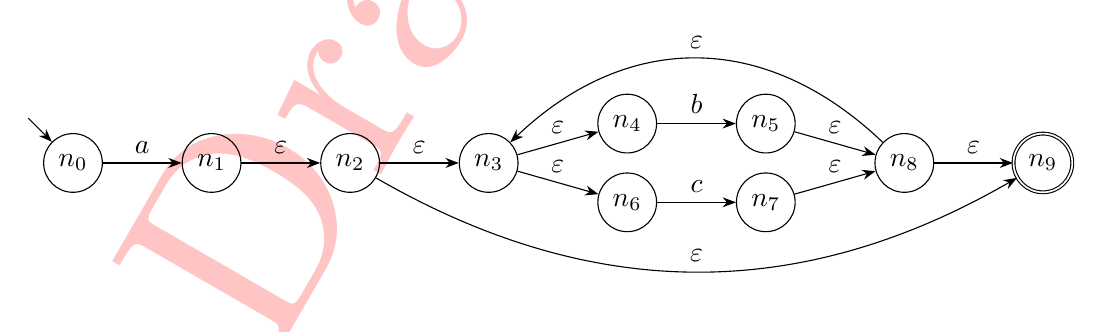
\begin{tikzpicture}[doublecircle/.style={circle,draw,double,minimum size=11pt}, state/.style={circle,draw,minimum size=12pt}, ->, >=Stealth, node distance=1cm]
        \node[state] (q0) {$n_0$};
        \node[state, right=of q0] (q1) {$n_1$};
        \node[state, right=of q1] (q2) {$n_2$};
        \node[state, right=of q2] (q3) {$n_3$};
        \node[state, right=of q3, yshift=0.5cm] (q4) {$n_4$};
        \node[state, right=of q4] (q5) {$n_5$};
        \node[state, right=of q3, yshift=-0.5cm] (q6) {$n_6$};
        \node[state, right=of q6] (q7) {$n_7$};
        \node[state, right=of q7, yshift=0.5cm] (q8) {$n_8$};
        \node[doublecircle, right=of q8] (q9) {$n_9$};

        \draw ($(q0.north west) + (-0.3cm, 0.3cm)$) to (q0);
        \path (q0) edge node[above] {$a$} (q1);
        \path (q1) edge node[above] {$\varepsilon$} (q2);
        \path (q2) edge node[above] {$\varepsilon$} (q3);
        \path (q3) edge node[above] {$\varepsilon$} (q4);
        \path (q4) edge node[above] {$b$} (q5);
        \path (q3) edge node[above] {$\varepsilon$} (q6);
        \path (q6) edge node[above] {$c$} (q7);
        \path (q5) edge node[above] {$\varepsilon$} (q8);
        \path (q7) edge node[above] {$\varepsilon$} (q8);
        \path (q8) edge node[above] {$\varepsilon$} (q9);
        \path (q2) edge [bend right] node[above] {$\varepsilon$} (q9);
        \draw (q8) .. controls ($(q5.north)+(0, 0.8cm)$) and ($(q4.north)+(0, 0.8cm)$) .. (q3) node[midway,above] {$\varepsilon$};
        %\path (q8) edge [bend right, looseness=1.5] node[above] {$\varepsilon$} (q3);
    \end{tikzpicture}
    \caption{由正则表达式 $a(b|c)^*$ 构造的 NFA 图}\label{fig:NFA-example}
\end{figure}

\subsection{NFA→DFA:子集构造算法}
由于 NFA 的一个状态可能对应多条出边,具有不确定性,我们用\Emph{子集构造算法}来把 NFA 转化为 DFA。

\begin{itemize}[leftmargin=1.5cm]
  \item 仿照 BFS 算法,在每次迭代中不断地将队头状态 $q$ 移出,并形成新的闭包,作为新的状态 $t$ 加入队列中。
  \item NFA 的结点用 $n$ 表示,DFA 的状态用 $q$ 表示。状态是结点的集合。
  \item 结点的闭包,指一个结点不输入任何字符即可达到的结点集合。
  \item $\delta$ 表示迁移函数,$\delta(q,c)$ 表示状态 $q$ 包含的所有结点经过字符 $c$ 之后转移得到的闭包之集合。\Notes{(比如状态 $\delta(q_0,a) = \delta(n_0,a) = n_1$,$\mathrm{e\_closure}(n_1) = \{n_1,n_2,n_3,n_4,n_6,n_9\}$。)}
  \item $\varepsilon$-闭包(\verb!eps_closure!)可以用 DFS 算法或 BFS 算法计算,比较简单。
\end{itemize}

\begin{lstlisting}
q0 <- eps_closure(n0) // n0的闭包
Q <- {q0}
workList <- q0
while (workList != [])
    remove q from workList
    foreach (character c)
        t <- e_closure (delta(q, c)) // q所包含的所有结点经字符c转移后的闭包
        D[q, c] <- t
        if (t\not\in Q)
            add t to Q and workList
\end{lstlisting}

图 \ref{fig:NFA-example} 中的表达式 $a(b|c)^*$ 转移得到的闭包如下:
\begin{align*}
    n_0(q_0) & \xrightarrow{a} \{n_1, n_2, n_3, n_4, n_6, n_9\} := q_1 \\
    q_1 &\xrightarrow{b} \{n_5, n_8, n_9, n_3, n_4, n_6\} := q_2 \\
    q_2 &\xrightarrow{c} \{n_7, n_8, n_9, n_3, n_4, n_6\} := q_3 \\
\end{align*}

经过迭代,得到的 DFA 如下图 \ref{fig:DFA-example} 所示。所有包含终止结点 $n_9$ 的状态都算作终结状态。
\begin{figure}[htb]
    \centering
    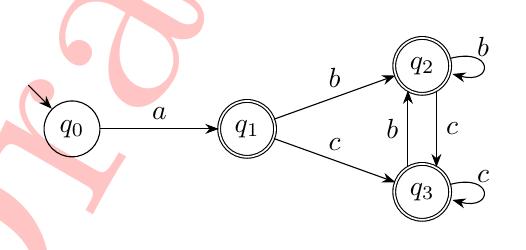
\begin{tikzpicture}[doublecircle/.style={circle,draw,double,minimum size=11pt}, state/.style={circle,draw,minimum size=12pt}, ->, >=Stealth, node distance=1.5cm]
        \node[state] (q0) {$q_0$};
        \node[doublecircle, right=of q0] (q1) {$q_1$};
        \node[doublecircle, right=of q1, yshift=0.8cm] (q2){$q_2$};
        \node[doublecircle, right=of q1, yshift=-0.8cm] (q3){$q_3$};

        \draw ($(q0.north west) + (-0.3cm, 0.3cm)$) to (q0);
        \path (q0) edge node[above] {$a$} (q1);
        \path (q1) edge node[above] {$b$} (q2);
        \path (q1) edge node[above] {$c$} (q3);
        \path (q2) edge [loop right] node[above] {$b$} (q2);
        \path (q3) edge [loop right] node[above] {$c$} (q3);
        \path (q3) edge [bend left, looseness=0] node[left] {$b$} (q2);
        \path (q2) edge [bend left, looseness=0] node[right] {$c$} (q3);
    \end{tikzpicture}
    \caption{由 $a(b|c)^*$ 几经转化得到的 DFA 图}\label{fig:DFA-example}
\end{figure}

子集构造算法的深入讨论:

\begin{itemize}[leftmargin=1.5cm]
  \item 这种算法属于\Emph{「不动点算法」}类型,即当算法不再产生新状态时逐渐停止。
  \item 决定算法能停止的关键是:状态有限。
  \item 对 $N$ 个结点的 NFA 图,其至多有 $2^N$ 种可能的状态。最坏时间复杂度 $O(2^N)$。但由于不是每个子集都会出现,所以该算法还是比较高效的。\Notes{(在这个例子中,最多有 512 种状态,但其实只出现了 4 个状态。)}
\end{itemize}

\subsection{DFA→词法分析器代码:Hopcraft最小化算法}
DFA 具有确定性,到了这一步其实可以算是完成了词法分析。但是有的 DFA 规模较大,不利于语法分析,因此我们可以用 \Emph{Hopcraft 算法}实现 DFA 的最小化。这个算法的介绍的代码比较「模糊」。

Hopcraft 采用等价类思想,初始时将所有状态并入一个大集合,不断地将状态集切分为非终态集合 $N$ 和终态集合 $A$。当不能再切分时算法停止,因此该算法也属于「不动点算法」。时间复杂度大致是 $O(n)$。

\begin{lstlisting}
split(S)
    foreach (character c)
        if (c can split S)
            split S into T1, …, Tk
hopcroft ()
    split all nodes into N, A
        while (set is still changes)
            split(S)
\end{lstlisting}

示例:图 \ref{fig:DFA-example} 中的 DFA 最小化后得到的新 DFA 如下图 \ref{fig:DFAmin-example} 所示:
\begin{figure}[htb]
    \centering
    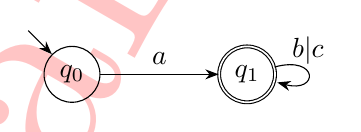
\begin{tikzpicture}[doublecircle/.style={circle,draw,double,minimum size=11pt}, state/.style={circle,draw,minimum size=12pt}, ->, >=Stealth, node distance=1.5cm]
        \node[state] (q0) {$q_0$};
        \node[doublecircle, right=of q0] (q1) {$q_1$};

        \draw ($(q0.north west) + (-0.3cm, 0.3cm)$) to (q0);
        \path (q0) edge node[above] {$a$} (q1);
        \path (q1) edge [loop right] node[above] {$b|c$} (q1);
    \end{tikzpicture}
    \caption{由 $a(b|c)^*$ 几经转化得到的最小化 DFA 图}\label{fig:DFAmin-example}
\end{figure}

\subsection{词法分析的驱动代码}
有了最小化的 DFA,就可以用关联矩阵实现。比如图 \ref{fig:DFAmin-example} 的 DFA 可用以下矩阵实现,这时可以用 $table[0][a]=1$ 表示在 $q_0$ 状态下接受字符 $a$。留空的部分表示 \ERROR 错误信息。
\begin{equation*}
    \kbordermatrix{
          & a & b & c \\
      q_0 & 1 &  & \\
      q_1 &  & 1 & 1 \\
    }
\end{equation*}

典型的词法分析驱动代码,依靠关联矩阵更新当前状态,并通过栈的记录,使得读到 \ERROR 状态时能够正确地退栈。代码中的 \verb!ACCEPT! 指终结状态。
\begin{lstlisting}
nextToken()
    state = 0
    stack = []
    while (state!=ERROR)
        c = getChar()
        if (state is ACCEPT) //当前状态为终结状态时,清栈
            clear(stack)
        push(state)
        state = table[state][c]
    while(state is not ACCEPT)
        state = pop();
        rollback();
\end{lstlisting}

举例:对图 \ref{fig:DFAmin-example} 的 DFA,处理字符串 \verb!ab#! 。
\begin{enumerate}[leftmargin=1.5cm]
    \item 初始时,栈为空。
    \item $state=q_0$,$c=$\verb!a!,保留栈中元素,$q_0$ 进栈,此时 $state=table[q_0][a]=q_1$,$stack=[q_0]$。
    \item $state=q_1$,$c=$\verb!b!,清栈,$q_1$ 进栈,此时 $state = table[q_1][b] = q_1$,$stack=[q_1]$。
    \item $state=q_1$,$c=$\verb!#!,清栈,$q_1$ 进栈,此时 $state = table[q_1][\#] = \ERROR$,$stack=[q_1]$。退出这个循环。
    \item \ERROR 状态不是终结状态,退栈一次,$state=q_1$,并回滚一个字符。
    \item $q_1$ 状态是终结状态,程序结束。词法分析器接受字符串中的 \verb!ab!,下次分析从 \verb!#! 开始。
\end{enumerate}

上述代码遵循「最长匹配」。在识别关键字 \verb!if! 和标识符 \verb!ifif! 的 DFA 例子中,如果读到了 \verb!ifif!,则会认定为标识符 \verb!ifif!,不会把 \verb!if! 切分出来。

还可以用跳转表的方式来实现词法分析,此时不使用关联矩阵,但需要每个状态各写一个跳转函数,适用于状态数量较少的 DFA。

\begin{lstlisting}
nextToken()
    state = 0
    stack = []
    goto q0
q0:
    c = getChar()
    if (state is ACCEPT)
        clear (stack)
    push (state)
    if (c==‘a’)
        goto q1
q1:
    c = getChar()
    if (state is ACCEPT)
        clear (stack)
    push (state)
    if (c==‘b’||c==‘c’)
        goto q1
\end{lstlisting}

\section{语法分析·大纲}
\subsection{语法分析的任务}
语法分析也位于「前端」部分,其输出作为语义分析的输入。语法分析的任务是将\Emph{记号序列}翻译为\Emph{抽象语法树}。

语法分析器做两件事:处理语法错误、构建语法树。

语法分析历史背景:「乔姆斯基文法体系」,上层包含下层。
\begin{itemize}[itemsep=0pt, parsep=0pt, leftmargin=1.5cm]
    \item 0 型文法:自然语言
    \item 1 型文法:上下文有关文法(语义分析的对象)
    \item 2 型文法:上下文无关文法(语法分析的对象)
    \item 3 型文法:正则表达式(词法分析的对象)
\end{itemize}

\subsection{上下文无关文法}
\Emph{上下文无关文法}的形式定义:$G = (T,N,P,S) =$ (终结符集,非终结符集,产生式规则,开始符)。

文法推导,就是不断地用产生式右部替换左部,直到不再出现非终结符。得到的符号串称为「句子」。
\begin{itemize}[itemsep=0pt, parsep=0pt, leftmargin=1.5cm]
    \item 最左推导:在产生式右部,每次选择\Emph{最左侧}的非终结符替换。
    \item 最右推导:在产生式右部,每次选择\Emph{最右侧}的非终结符替换。
\end{itemize}

\subsection{分析树与二义性文法}
给定文法 $G$ 和句子 $s$,问是否存在一个对 $s$ 的推导?这是语法分析要解决的问题。

\Emph{分析树}是描述推导过程的数据结构。如根据以下文法
\begin{equation}\label{eq:G-1}
\begin{split}
  E \to \ & num \\
    \OR  & id \\
    \OR  & E+E \\
    \OR  & E*E
\end{split}
\end{equation}
推导句子 $s$:\verb!3 + 4 * 5!,即使都采用\Emph{最左推导},仍然存在以下 2 种推导方式:

\begin{figure}[htb]
\newcommand\hightlight[1]{\textcolor{darkcyan}{#1}}
\begin{minipage}[t]{.49\textwidth}
    \centering
    \begin{align*}
        E\to & \hightlight{E} + E \\
        \to  & 3 + \hightlight{E} \\
        \to  & 3+\hightlight{E}*E \\
        \to  & 3+4*\hightlight{E} \\
        \to  & 3+4*5 \\
    \end{align*}
    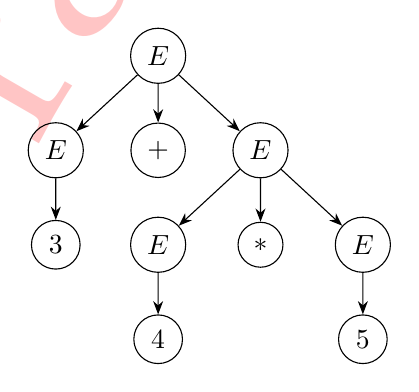
\begin{tikzpicture}[
          level 1/.style={sibling distance=13mm},
          level 2/.style={sibling distance=13mm},
          level distance=12mm,
          edge from parent/.style={->,draw},
          every node/.style={circle, draw, minimum size=1em},
          >=Stealth
        ]
        \node [circle, draw] (root) {$E$}
          child {node [circle, draw] (c1) {$E$}
            child {node [circle, draw] (c11) {3}
            }
          }
          child {node [circle, draw] (c2) {$+$}
          }
          child {node [circle, draw] (c3) {$E$}
            child {node [circle, draw] (c31) {$E$}
                child {node [circle, draw] (c311) {4}}
            }
            child {node [circle, draw] (c32) {$*$}
            }
            child {node [circle, draw] (c33) {$E$}
                child {node [circle, draw] (c331) {5}}
            }
          };
        \end{tikzpicture}
\end{minipage}
\begin{minipage}[t]{.49\textwidth}
    \centering
    \begin{align*}
        E\to & \hightlight{E} * E \\
        \to  & \hightlight{E}+E*E \\
        \to  & 3+\hightlight{E}*E \\
        \to  & 3+4*\hightlight{E} \\
        \to  & 3+4*5 \\
    \end{align*}
    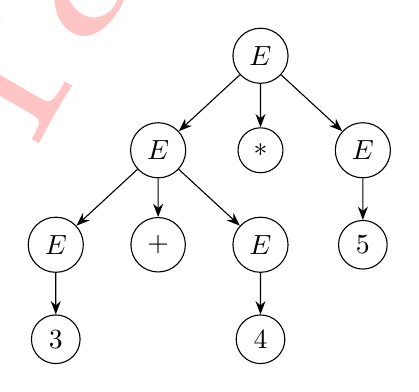
\begin{tikzpicture}[
          level 1/.style={sibling distance=13mm},
          level 2/.style={sibling distance=13mm},
          level distance=12mm,
          edge from parent/.style={->,draw},
          every node/.style={circle, draw, minimum size=1em},
          >=Stealth
        ]
        \node [circle, draw] (root) {$E$}
          child {node [circle, draw] (c1) {$E$}
            child {node [circle, draw] (c11) {$E$}
                child {node [circle, draw] (c111) {3}}
            }
            child {node [circle, draw] (c12) {$+$}
            }
            child {node [circle, draw] (c13) {$E$}
                child {node [circle, draw] (c131) {4}}
            }
          }
          child {node [circle, draw] (c2) {$*$}
          }
          child {node [circle, draw] (c3) {$E$}
            child {node [circle, draw] (c31) {5}
            }
          };
        \end{tikzpicture}
\end{minipage}
    \caption{句子 \texttt{3 + 4 * 5} 的两种推导方式和推导树}\label{fig:tuidao}
\end{figure}

\begin{itemize}[itemsep=0pt, parsep=0pt, leftmargin=1.5cm]
    \item 左边的推导树实际上是 $3+(4*5)$,乘法优先级更高。(先序遍历)
    \item 右边的推导树实际上是 $(3+4)*5$,加法优先级更高。
\end{itemize}
本例体现了计算顺序不同产生的二义性。

给定文法 $G$,如果存在句子 $s$,它有两棵不同的分析树,那么称 $G$ 是\Emph{二义性文法}。解决二义性文法的一个方案是,文法的重写。比如把上述文法 \eqref{eq:G-1} 改写成以下形式,强制将推导树的乘法部分置于加法部分的后继,使推导树的乘法优先级更高,这样就消除了二义性。\Notes{(注:本文档出现的文法可能都会多次使用到,所以用标号 \eqref{eq:G-1}\eqref{eq:G-2} 等来引用。)}
\begin{equation}\label{eq:G-2}
\begin{split}
   E\to\  & E+T \\
    \OR & T \\
   T\to\  & T*F \\
    \OR & F \\
   F\to\  & num\\
    \OR & id
\end{split}
\end{equation}
通过文法 \eqref{eq:G-2} 推导句子 \verb!3 + 4 * 5! 只可能是 $3+(4*5)$ 了。

此外,语法分析不仅要能回答一个句子是「正确的」,还要能鉴别一个句子是「错误的」。以下的章节中列出了语法分析的两个类别:自顶向下分析、自底向上分析。

\section{语法分析·自顶向下}
\subsection{自顶向下分析}\label{subsec:自顶向下分析}
从开始符入手推导句子,即为\Emph{自顶向下分析},对应于分析树自顶向下构造的顺序。

这种分析方式需要不断回溯,效率较低,通常是 $O(2^n)$ 的。原始的自顶向下分析算法如下所示(应该并不重要,重要的是改进的算法):
\begin{lstlisting}
tokens[];     // all tokens
i=0;
stack = [S];  // S是开始符号
while (stack != [])
    if (stack[top] is a terminal t)
        if (t==tokens[i++])
            pop();
        else
            backtrack();
    else if (stack[top] is a nonterminal T)
        pop();
        push(the next right hand side of T);
\end{lstlisting}


使用 LL(1) 算法生成\Emph{分析表}后,可以采用分析表来改进自顶向下分析算法。代码详见 \ref{subsec:LL(1)} 小节结尾的代码。


\subsection{递归下降分析}
\Emph{递归下降分析}也称为预测分析,能在线性时间内完成。用一个前看符号指导产生式规则的选择。可能需要具体问题具体编码。比如,对课上常提的「羊吃草」文法:
\begin{equation}\label{eq:G-NVN}
\begin{split}
   S\to\  & NVN \\
   N\to\  & s \OR t \OR g \OR w \\
   V\to\  & e \OR d
\end{split}
\end{equation}
可构造如下的递归下降分析代码:

\begin{lstlisting}
parse_S()
    parse_N()
    parse_V()
    parse_N()
parse_N()
    token = tokens[i++] // 依次读取记号序列的记号
    if (token=='s' || token=='t' || token=='g' || token=='w')
        return; // 有适合的前看符号,就返回上级函数,否则报错
    error("...");
parse_V()
    token = tokens[i++]
    if (token=='e' || token=='d')
        return;
    error("...");
\end{lstlisting}

再比如对算术表达式文法 \eqref{eq:G-2} 的递归下降分析:
\begin{lstlisting}
parse_E()
    parse_T()
    token = tokens[i++]
    while (token == '+')
        parse_T()
        token = tokens[i++]
parse_T()
    parse_F()
    token = tokens[i++]
    while (token == '*')
        parse_F()
        token = tokens[i++]
parse_F()
    token = tokens[i++]
    if(token==num || token==id)
        return;
    error("...");
\end{lstlisting}


\subsection{LL(1)算法}\label{subsec:LL(1)}
\Emph{LL(1) 算法}是一种自顶向下分析算法,其思路是从左(L)向右读入程序,最左(L)推导,采用一个(1)前看符号。LL(1) 算法的目标是生成分析表,以供自顶向下分析算法使用。

该算法需要求出每个非终结符的 \FIRST 集、\FOLLOW 集,以及每个产生式的 \FIRSTS 集。

\begin{tcolorbox}[colback=violet!5, colframe=violet, boxrule=1pt, breakable]
\begin{enumerate}
  \item \Emph{\NULLABLE 集}:
    假设 $X$ 为非终结符。$X\in \NULLABLE$,当且仅当 $X\to \varepsilon$ 或者 $X\to \beta_1\beta_2\cdots\beta_n$(其中每个 $\beta_i$ 均属于 \NULLABLE)。
  \item 非终结符的 \Emph{\FIRST 集}:
    \begin{equation*}
      \FIRST(A) = \{a\ |\ A\deduce aB\}
    \end{equation*}
    其中,$a\in \VT$(终结符),$B \in V^*$ (任意符号串),$\deduce$ 表示「经由任意次推导」。
  \item 非终结符的 \Emph{\FOLLOW 集}:
    \begin{equation*}
      \FOLLOW(A) = \{a\ |\ S\deduce \cdots Aa\cdots \}
    \end{equation*}
    其中 $S$ 为开始符号,$a\in \VT$(终结符)。
  \item 产生式的 \Emph{\FIRSTS 集}:对于产生式 $p:A\to \alpha$。
    \begin{itemize}
      \item 若 $\alpha\in\NULLABLE$,则 $\FIRSTS(p) = \FIRST(\alpha)\cup \FOLLOW(A)$;
      \item 若 $\alpha\notin\NULLABLE$,则 $\FIRSTS(p) = \FIRST(\alpha)$。
    \end{itemize}
\end{enumerate}

通俗解释:
\begin{itemize}
  \item \FIRST$(A)$ 就是非终结符 $A$ 经任意次推导后,可能得到的开头终结符的集合。
  \item \FOLLOW$(A)$ 就是开始符 $S$ 经任意次推导后,$A$ 可能紧接着的终结符的集合。
  \item \FIRSTS$(p)$ 就是产生式 $p$ 经任意次推导后,可能得到的开头终结符的集合。
\end{itemize}

\Notes{(注:课本上的这几个集合有特殊的规定:(i) 当 $\alpha$ 能推导出 $\varepsilon$,则规定 $\varepsilon\in\FIRST(\alpha)$;(ii) 若存在 $S$ 能推导出 $A$,则规定结束符 $\$\in \FOLLOW(A)$;(iii) 若产生式 $p:A\to\alpha$ 的 $\alpha\in\NULLABLE$,则 $\FIRSTS(p) = (\FIRST(\alpha)-\{\varepsilon\})\cup \FOLLOW(A)$;(iv) \FIRSTS 集也称为 \textsc{Select} 集。本文档与PPT和老师讲解内容同步,不采用这些规定。)}

\end{tcolorbox}

\paragraph{\NULLABLE 集} 找到可能推出空记号 $\varepsilon$ 的非终结符,可以直接利用定义。
\begin{lstlisting}
NULLABLE = {};
while (NULLABLE is still changing)
    foreach (production `$p: X\to \beta$`)
    if (`$\beta$` == `$\varepsilon$`)  //能直接推出空记号
        NULLABLE `$\cup$`= {`$X$`}
    if (`$\beta$` == `$Y_1\cdots Y_n$`) //每一项都是属于NULLABLE的非终结符
        if (`$Y_1\in$`NULLABLE && … && `$Y_n\in$`NULLABLE)
            NULLABLE `$\cup$`= {`$X$`}
\end{lstlisting}

\paragraph{\FIRST 集} 找到一个非终结符所有可能推出的第一个终结符,可以用归纳法。假设产生式是 $N\to \beta_1\beta_2\cdots\beta_n$,$\FIRST(N)$ 从 $\beta_1$ 开始不断地往后取各个符号的 \FIRST 的并集,除非遇到了「终结符」或「不能推出空记号的非终结符」就停止取并。\Notes{(事实上,「终结符」和「不能推出空记号的非终结符」在求解 \FIRST、\FOLLOW、\FIRSTS 集时是等效的。)}
\begin{lstlisting}
foreach (nonterminal N)
    FIRST(N) = {}
while(some set is changing)
    foreach (production `$p: N\to\beta_1\beta_2\cdots\beta_n$`)  // 外层对产生式迭代
        foreach (`$\beta_i$` from `$\beta_1$` up to `$\beta_n$`) // 内层对每个记号迭代(正序)
            if (`$\beta_i$`== `$a$`) // 遇到终结符停止取并
                FIRST(`$N$`) `$\cup$`= {`$a$`};
                break;
            if (`$\beta_i$`== `$M$`)
                FIRST(`$N$`) `$\cup$`= FIRST(`$M$`);
                if (`$M$` is not in NULLABLE) // 遇到不能推出空记号的停止取并
                    break;
\end{lstlisting}

\paragraph{\FOLLOW 集} 找到一个非终结符的所有前看符号,有些麻烦。假设产生式是 $N\to \beta_1\beta_2\cdots\beta_n$,$\FOLLOW(N)$ 从 $\beta_n$ 开始往前更新 $temp$。$temp$ 是当前存储的「前看符号集合」。
\begin{itemize}
  \item $temp$ 在开始时先赋予 $N$ 当前的前看符号。
  \item 每遇到一次非终结符 $M$,则表明 $M$ 能遇到的前看符号包含 $temp$,这时更新 $\FOLLOW(M) \cup= temp$。
  \item 接下来往前挪动一个字符 $\beta_i$。$\beta_i$ 能不能推出 $\varepsilon$,决定了 $temp$ 是要先清空再赋予 $\FIRST(\beta_i)$,还是直接赋予 $\FIRST(\beta_i)$。\Notes{(打个比方,不能推出 $\varepsilon$ 的 $\beta_i$ 是一座山,$temp$ 翻山越岭前得先卸载自己的包袱;能推出 $\varepsilon$ 的 $\beta_i$ 是一块平地,$temp$ 不需要卸载包袱就可以自由通行。通行以后还需要多运输 $\FIRST(\beta_i)$ 的货物。)}
\end{itemize}

\begin{lstlisting}
foreach (nonterminal N)
    FOLLOW(N) = {}
while(some set is changing)
    foreach (production `$p: N\to\beta_1\beta_2\cdots\beta_n$`) // 外层对产生式迭代
    temp = FOLLOW(`$N$`) // temp在开始时先赋予N当前的前看符号,别忘了
    foreach (`$\beta_i$` from `$\beta_n$` down to `$\beta_1$`) // 内层对每个记号迭代(倒序)
        if (`$\beta_i$`== `$a$`)
        temp = {`$a$`}
        if (`$\beta_i$`== `$M$`)
            FOLLOW(`$M$`) `$\cup$`= temp
            if (`$M$` is not NULLABLE)
                temp = FIRST(`$M$`)
            else temp `$\cup$`= FIRST(`$M$`)
\end{lstlisting}

\paragraph{\FIRSTS 集} 找到一条产生式所有可能的第一个终结符,也用归纳法。假设产生式是 $p:N\to \beta_1\beta_2\cdots\beta_n$,$\FIRSTS(p)$ 从 $\beta_1$ 开始不断地往后取各个符号的 \FIRST 的并集,除非遇到了「终结符」或「不能推出空记号的非终结符」就停止取并。此外,如果到了最后一个记号 $\beta_n$ 还未停止,那么还需要额外并上 $\FOLLOW(N)$。\Notes{(因此,如果产生式是 $p:N\to\varepsilon$,那么 $\FIRSTS(p)=\FOLLOW(N)$。)}
\begin{lstlisting}
foreach (production p)
    FIRST_S(p) = {}
calculte_FIRST_S(production `$p: N\to\beta_1\beta_2\cdots\beta_n$`)
    foreach (`$\beta_i$` from `$\beta_1$` up to `$\beta_n$`)
        if (`$\beta_i$`== `$a$`)
            FIRST_S(`$p$`) `$\cup$`= {`$a$`}
            return;
        if (`$\beta_i$`== `$M$`)
            FIRST_S(`$p$`) `$\cup$`= FIRST(`$M$`)
            if (`$M$` is not NULLABLE)
                return;
    FIRST_S(`$p$`) `$\cup$`= FOLLOW(`$N$`) // 注意这一行在读完整条产生式之后才可能执行
\end{lstlisting}

\paragraph{LL(1) 分析表} 有了所有产生式的 \FIRSTS 集,就可以构造 LL(1) 分析表了。该分析表用于语法分析驱动代码(自顶向下分析程序)。

\paragraph{LL(1) 分析器} 完整的 LL(1) 自顶向下分析程序(语法分析驱动代码)就是这一段。算法的核心在于\Emph{ $table[T,\ token_i]$},表示栈顶为 $T$,匹配到记号 $token_i$ 时,使用的生成式序号。因此进栈的是对应生成式的右部。
\begin{lstlisting}
tokens[];     // all tokens
i=0;
stack = [S];  // S是开始符号
while (stack != [])
    if (stack[top] is a terminal t)
        if (t==tokens[i++])
            pop();
        else
            error("..."); // 不回溯
    else if (stack[top] is a nonterminal T)
        pop();
        push(the correct right hand side of T: `$table[T,\ token_i]$`); //查表得到的产生式右部进栈
\end{lstlisting}

最后,我们的文法必须满足一个条件才能成为 LL(1) 文法:对每个非终结符 $A$ 的任意两条产生式 $A\to\alpha$、$A\to\beta$(其中 $\alpha,\beta$ 不同时 $\deduce\varepsilon$),需要满足条件:
\begin{equation*}
    \FIRSTS(A\to\alpha)\ \cap\ \FIRSTS(A\to\beta) = \varnothing
\end{equation*}
反映在分析表上,就是看是否存在同一表项中至少有 2 个产生式(即构成冲突)。如果没有冲突,那就是 LL(1) 文法;如果有冲突,就要对文法进行等价变换,比如消除左递归和提取左公因子。




\section{语法分析·自底向上}
\subsection{LR(0)算法}
语法分析还可以使用自底向上分析,其思想是最右推导的逆过程。这时有两个主要操作:\Emph{移进}和\Emph{归约}。
\begin{itemize}[leftmargin=1cm]
  \item 移进:一个记号进栈。
  \item 归约:若栈顶的若干个符号刚好满足一条产生式的右部,则这些符号退栈,换产生式左部进栈。
\end{itemize}

核心的问题是,如何确定移进和归约的时机?这时就有了 \Emph{LR(0) 算法}。我们用点标记来记录读入了多少输入。每一个带上了点标记的产生式都可以算做一个「LR(0) 项目」。例如:LR(0) 项目 $[S\to xx\D T]$ 表示栈中已存在 $xx$,如果遇到 $T$ 则产生移进。

\begin{description}[leftmargin=1cm]
  \item[拓广文法] 此时要分析的文法变为「拓广文法」,即对原文法 $G[S]$ 增设一条产生式 $S'\to S\$ $ 变为文法 $G'[S']$,有一个明显的结束符 \$。
  \item[闭包计算] 在每个状态中,若遇到了形如 $S\to\D A\dots$ 的产生式(圆点紧接着非终结符),则需要把所有以该非终结符 $A$ 开头的产生式也加入到同一状态中。
  \item[分析表填写] LR(0) 分析表取决于 DFA 状态图,移进一个终结符时写入 \ACTION 表,移进一个非终结符时写入 \GOTO 表,归约一条产生式(或接受整个字符串)时写入 \ACTION 表。
  \item[下标含义] 移进项和归约项的下标含义不同。如移进项 $s_2$ 表示「移进到状态 2」,归约项 $r_2$ 表示「用 2 号产生式归约」。
\end{description}


以下是 LR(0) 驱动代码。在栈中,一个符号紧接着一个状态数字,成对出现,称为「双栈」。
\begin{lstlisting}
stack = []
push ($)      // $: 结束符
push (1)      // 1: 初始状态(也可能是0)
while (true)
    token t = nextToken() // t仅在移进时向前移动,归约时原地停留
    state s = stack[top]
    if (ACTION[s, t] == '`$s_i$`') // 移进
        push (t); push (i)
    else if (ACTION[s, t] == '`$r_j$`') // 归约
        pop (the right hand of production `$j: X \to \beta$`)
        state s = stack[top]
        push (X);
        push (GOTO[s, X]);
    else error (…)
\end{lstlisting}

此外,分析表可以用算法自动构造,也可以通过 DFA 状态图手动转化。自动构造算法用到了 \verb!goto! 和 \verb!closure! 函数。

\subsection{SLR(1)算法}

LR(0) 算法能分析的文法有限,因为它可能会有两种冲突:
\begin{description}
    \item[移进—归约冲突] 对于某一状态,若其既可对应移进操作,也可对应归约操作,则存在冲突。分析表上的一个单元格需要同时具备 $s_i$ 和 $r_j$。
    \item[归约—归约冲突] 对于某一状态,若存在多个归约项目,且对应的产生式不同,则存在冲突。分析表上的一个单元格需要同时具备 $r_j$ 和 $r_{j'}$。
\end{description}
而如果换成 \Emph{SLR(1) 算法},或许可以利用一个前看符号(\FOLLOW 集)来规避冲突。

SLR(1) 算法与 LR(0) 仅在归约操作有区别:对于状态 $i$ 的归约项目 $X\to \alpha\D$,并不对 \ACTION 表上的每一列添加归约项,而是仅对满足 $y\in \FOLLOW(X)$ 的 $y$ 列添加归约项。\Notes{(此外,如果一状态有多个归约项目如 $A\to\alpha\D$、$B\to\beta\D$,这时还要满足 $\FOLLOW(A)\cap\FOLLOW(B)=\varnothing$,否则分析表上仍有一个单元格同时具备两个归约操作,冲突无法消解。)}

\subsection{LR(1) 算法}
即使是 SLR(1) 算法也可能冲突,这里引入 \Emph{LR(1) 算法}。LR(1) 的项目相比 LR(0) 添加了前看符号 $a$,如 $[X\to \alpha\D\beta, \ a]$。

\begin{itemize}
  \item 闭包计算:对项目 $[X\to \dots\D Y \beta,\ a]$,添加 $[Y\to \D\dots,\ b]$,其中前看符号 $b\in \FIRSTS(\beta a)$。\Notes{(用 \FIRSTS 是因为 $\beta a$ 是多记号的产生式。)}
  \item 归约方式:对归约项 $[X\to \alpha\D, \ a]$,仅对 $a$ 列写入归约规则「归约至产生式 $X\to\alpha$」。
\end{itemize}

本算法了解即可。


\subsection{文法的判别}
要判断一个文法是否是某种特定的文法(LL(1)、LR(0)、SLR(1)等),可以用该种文法对应的\Emph{分析表}来分析,观察分析表上是否有冲突。若无冲突,则可说明待判别文法是要求的特定文法;否则不是要求的特定文法。此外,若一文法是 LR(0) 文法,则其一定也是 SLR(1) 文法,反之不然。

\begin{table}[htb]
  \centering
  \begin{tabular}{|c|p{.7\textwidth}|}
    \hline
    文法 & 判别方式 \\
    \hline
    LL(1) & 对每个非终结符 $A$ 的任意两条产生式 $p:A\to\alpha$ 和 $q:A\to\beta$,需要满足 $\FIRSTS(p)\cap\FIRSTS(q)=\varnothing$ \\
    \hline
    LR(0) & 状态图中不存在移进—归约冲突和归约—归约冲突 \\
    \hline
    SLR(1) & 同一状态的任意两个归约项目 $A\to\alpha\D$、$B\to\beta\D$,需要满足 $\FOLLOW(A)\cap\FOLLOW(B)=\varnothing$ \\
    \hline
  \end{tabular}
  \caption{文法的判别}\label{tab:judgement}
\end{table}



\section{抽象语法树}
\subsection{语法制导翻译}
\Emph{语法制导翻译}是编译器进行语法分析时的附加工作,其基本思想是在每个产生式规则附加一条动作,在产生式归约时执行。换言之,当产生式右部分析完毕,开始归约的时候,这些动作就开始执行。

在 LR 分析中,在分析栈上维护三元组 \verb!<symbol, value, state>!。

示例:PPT 上的 $E \to E+E \OR n$。其中的 \verb!$$! 表示产生式左部,\verb!$1!,\verb!$3! 分别表示产生式右部的第 1 个、第 3 个记号(即左数第 2 个 $E$ 和第 3 个 $E$)。本例语法制导翻译的功能是,计算加法表达式的值。

\subsection{抽象语法树}
\Emph{抽象语法树}是对分析树的简化,略去优先级、结合性、记号写法等无关紧要特征,只保留语法结构,以及每个语法结构在文件中的\Emph{位置}(行号、列号等)。抽象语法树是语法分析部分的最终输出。以下是表达式 $3+(4*5)$ 的抽象语法树例子。

\begin{figure}[htb]
  \begin{minipage}[t]{.49\textwidth}
  \centering
    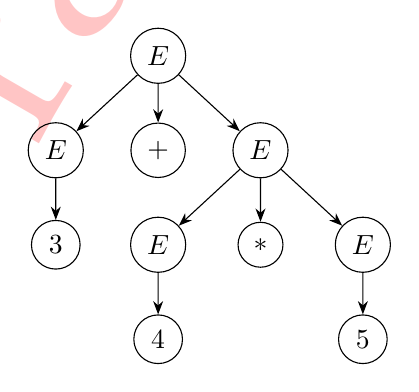
\begin{tikzpicture}[
      level 1/.style={sibling distance=13mm},
      level 2/.style={sibling distance=13mm},
      level distance=12mm,
      edge from parent/.style={->,draw},
      every node/.style={circle, draw, minimum size=1em},
      >=Stealth
    ]
    \node [circle, draw] (root) {$E$}
      child {node [circle, draw] (c1) {$E$}
        child {node [circle, draw] (c11) {3}
        }
      }
      child {node [circle, draw] (c2) {$+$}
      }
      child {node [circle, draw] (c3) {$E$}
        child {node [circle, draw] (c31) {$E$}
            child {node [circle, draw] (c311) {4}}
        }
        child {node [circle, draw] (c32) {$*$}
        }
        child {node [circle, draw] (c33) {$E$}
            child {node [circle, draw] (c331) {5}}
        }
      };
    \end{tikzpicture}
  \end{minipage}
  \begin{minipage}[t]{.49\textwidth}
  \centering
    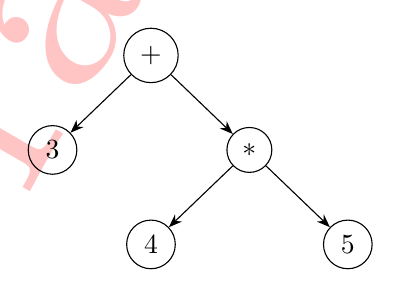
\begin{tikzpicture}[
      level 1/.style={sibling distance=25mm},
      level 2/.style={sibling distance=25mm},
      level distance=12mm,
      edge from parent/.style={->,draw},
      every node/.style={circle, draw, minimum size=1em},
      >=Stealth
    ]
    \node [circle, draw] (root) {$+$}
      child {node [circle, draw] (c1) {$3$}
      }
      child {node [circle, draw] (c2) {$*$}
        child {node [circle, draw] (c21) {$4$}
        }
        child {node [circle, draw] (c22) {$5$}
        }
      };
    \end{tikzpicture}
  \end{minipage}
  \caption{表达式 $3+(4*5)$ 的分析树(左)与抽象语法树(右)}\label{fig:分析树与抽象语法树}
\end{figure}

可以看到,表达式 $3+(4*5)$ 对应的抽象语法树的中序遍历 \verb!3+4*5! 即是它本身,后序遍历 \verb!345*+! 即是对应的逆波兰式。

\begin{verbatim}
    e1 = Exp_int_new(3)
    e2 = Exp_int_new(4)
    e3 = Exp_int_new(5)
    e4 = Exp_int_times(e2, e3)
    e5 = Exp_int_add(e1, e4)
\end{verbatim}

可以看到,编码这棵抽象语法树时采用了\Emph{后序遍历}的方法。

此外,对抽象语法树这个树形数据结构,可以实现很多工作,比如「优美打印」和树上的递归计算节点个数。以下是示例:从表达式到栈式计算机 Stack 的编译器(供参考):
\begin{lstlisting}
List all;
void compile (E e)
{
    switch (e->kind) {
        case E_INT: emit(push e->n); return;
        case E_ADD: compile(e->left); compile(e->right); emit(add); return;
        case E_TIMES: compile(e->left); compile(e->right); emit(times); return;
        default: error ("compiler bug");
    }
}
\end{lstlisting}

\Emph{考点}:抽象语法树和具体语法树的互化。

\section{语义分析}
\subsection{语义分析的任务}
\Emph{语义分析}也是上下文相关分析,用于检查诸如「变量先声明后使用」、「二元运算的两个操作数的类型要一致」此类的上下文相关问题。

\paragraph{实例:类型检查} 对以下文法
\begin{equation}\label{eq:G-type}
\begin{split}
   E\to\  & n \OR \text{true} \OR \text{false} \\
    \OR & E+E \\
    \OR & E \&\& E
\end{split}
\end{equation}
我们需要检查加法操作时的两个操作数均为 \verb!int! 类型,与操作时的两个操作数均为 \verb!bool! 类型。逻辑比较简单。

\begin{lstlisting}
enum type {INT, BOOL};
enum type check_exp (Exp_t e)
    switch(e->kind)
        case EXP_INT: return INT;
        case EXP_TRUE: return BOOL;
        case EXP_FALSE: return BOOL;
        case EXP_ADD:
            t1 = check_exp (e->left);
            t2 = check_exp (e->right);
            if (t1!=INT || t2!=INT)
                error ("type mismatch");
            else return INT;
        case EXP_AND: // 此块可能留作考题
            t1 = check_exp (e->left);
            t2 = check_exp (e->right);
            if (t1!=BOOL || t2!=BOOL)
                error ("type mismatch");
            else return BOOL;
\end{lstlisting}



\subsection{符号表}
\Emph{符号表}本质上是一种查找表,存储了每个变量的类型、作用域层级等信息。在数据结构层面,可以使用哈希表、红黑树等方式实现。

对简单问题,可以用一个哈希表来存储符号表。有新元素在作用域中定义时,插入表项;当有元素从作用域退出时,删除表项。

以下例子中,用 \verb!变量:(类型,作用域层级)! 的方式描述符号表,如 \verb!x:(INT,0)!。
\begin{lstlisting}
int x;          // [插入] x:(INT,0)
int f ()        // [插入] x:(INT,0), f:(INT,1)
{
    if (4) {
        int x;  // [插入] x:(INT,0), f:(INT,1), x:(INT,2)
        x = 6;
    }           // [删除] x:(INT,0), f:(INT,1)
    else {
        int x;  // [插入] x:(INT,0), f:(INT,1), x:(INT,2)
        x = 5;
    }           // [删除] x:(INT,0), f:(INT,1)
    x = 8;
}               // [删除] x:(INT,0)
\end{lstlisting}

符号表还可以处理名字空间(namespace),还可以每个类定义一个符号表。

以下是语义分析考虑的典型问题:
\begin{itemize}[itemsep=0pt, parsep=0pt,leftmargin=1.5cm]
  \item 类型检查
  \item 变量声明和定义
  \item 类型相容
  \item 错误诊断
  \item 代码翻译
\end{itemize}

\section{代码生成与优化}
代码生成是「后端」的一个过程。其主要任务是把\Emph{抽象语法树}翻译成\Emph{目标机器}上的代码。具体地:
\begin{itemize}[itemsep=0pt, parsep=0pt,leftmargin=1.5cm]
    \item 给数据分配计算资源
    \item 给代码选择指令
\end{itemize}

假设有一种 $\mathrm{C--}$ 语言的文法,在这一章会用到:
\begin{equation}\label{eq:C--}
\begin{split}
   P \to\  & D\ S \\
   D \to\  & T\ id;\ D \\
   \OR & \varepsilon \\
   T \to\ & \mathrm{int} \\
   \OR & \mathrm{bool} \\
   S \to\ & id=E \\
   \OR & \mathrm{printi}(E) \\
   \OR & \mathrm{printb}(E) \\
   E \to\ & n \OR id \OR \mathrm{true} \OR \mathrm{false} \\
   \OR & E+E \\
   \OR & E\operatorname{\&\&} E
\end{split}
\end{equation}

\subsection{代码生成·栈式计算机}
\Emph{栈式计算机}用栈来存储运算数,并和存储器做数据交换。栈式计算机有 7 条指令(详见PPT),其中的 \verb!load! 指令用于将数据从存储器移入栈,\verb!store! 指令用于将数据从栈移入存储器。

栈式计算机只支持 \verb!int! 类型数据,定义数据时给数据分配\Emph{内存}空间。读操作数的值时使用 \verb!load! 指令,修改操作数的值时使用 \verb!store! 指令。

\begin{itemize}[itemsep=0pt,parsep=0pt,leftmargin=1.5cm]
  \item \verb!int x! 改写为 \verb!.int!
  \item \verb!x = 10! 改写为 \verb!push 10, store x!
  \item \verb!z = x + y! 改写为 \verb!load x, load y, add, store z!
\end{itemize}

从 $\mathrm{C--}$ 语言到栈式计算机(目标机器),生成代码需要 5 个递归函数,对应 5 个非终结符:
\begin{lstlisting}
Gen_E(E e) // 表达式expression
    switch (e)
        case n: emit ("push n"); break;
        case id: emit ("load id"); break;
        case true: emit ("push 1"); break; // 栈式计算机只有int类型
        case false: emit ("push 0"); break;
        case e1+e2: Gen_E (e1); Gen_E (e2); emit ("add"); break;
        case e1&&e2: Gen_E (e1); Gen_E (e2); emit ("and"); break; // 已补全
Gen_S(S s) // 句子sentence
    switch (s)
        case id=e: Gen_E(e); emit("store id"); break;
        case printi(e): Gen_E(e); emit ("printi"); break;
        case printb(e): Gen_E(e); emit ("printb"); break;
Gen_T(T t) // 变量类型type
    switch (t)
        case int: emit (".int"); break;
        case bool: emit (".int"); break; // 栈式计算机只有int类型
Gen_D(T id; D) // 声明式declaration
    Gen_T (T);
    emit (" id");
    Gen_D (D);
Gen_P(D S) // 主程序program
    Gen_D(D);
    Gen_S(S);
\end{lstlisting}

\subsection{代码生成·寄存器式计算机}
\Emph{寄存器式计算机}用各个通用寄存器存储运算数,并和存储器做数据交换。这里假设寄存器数量有无穷多个。寄存器式计算机有 8 条指令(详见PPT),其中带 \verb![]! 的表示内存中的数。

寄存器式计算机这里同样只支持 \verb!int! 类型数据,定义数据时给数据分配\Emph{寄存器}空间。注意 \verb!movn! 和 \verb!mov! 指令的区别,前者有立即数,后者无立即数。
\begin{itemize}[itemsep=0pt,parsep=0pt,leftmargin=1.5cm]
  \item \verb!int! 直接改写为 \verb!.int!
  \item \verb!x = 10! 改写为 \verb!movn 10,r!;\verb!mov r,y!
  \item \verb!z = x + y! 改写为 \verb!add x,y,z!(如果 $x,y,z$ 都存储于寄存器)
  \item \verb!1 + 2! 改写为 \verb!movn 1,r1!;\verb!movn 2,r2!;\verb!add r1,r2,r3!(中间变量用临时寄存器存储)
\end{itemize}

从 $\mathrm{C--}$ 语言到寄存器式计算机(目标机器),生成代码也需要 5 个递归函数,对应 5 个非终结符,其中只有 \verb!Gen_E! 和 \verb!Gen_S! 有变化,另外 3 个函数与栈式计算机的无异。
\begin{itemize}[itemsep=0pt,parsep=0pt,leftmargin=1.5cm]
  \item \verb!Gen_E! 函数多了一个寄存器号作为返回值,在 \verb!Gen_S! 中使用到这个值。
  \item \verb!fresh()! 函数用来分配可用的寄存器并刷新其值。
  \item 处理 \verb!e1 && e2! 表达式时两个操作数都需要递归处理,不采取「短路效应」规则。
\end{itemize}
\begin{lstlisting}
R_t Gen_E(E e) // 表达式expression
    switch (e)
        case n:     r = fresh(); emit ("movn n, r"); return r;
        case id:    r = fresh(); emit ("mov id, r"); return r;
        case true:  r = fresh(); emit ("movn 1, r"); return r;
        case false: r = fresh(); emit ("movn 0, r"); return r;
        case e1+e2: r1 = Gen_E(e1); r2 = Gen_E(e2);
            r = fresh(); emit ("add r1, r2, r"); return r;
        case e1&&e2: r1 = Gen_E(e1); r2 = Gen_E(e2);
            r = fresh(); emit ("and r1, r2, r"); return r;
Gen_S(S s) // 句子sentence
    switch (s)
        case id=e:      r = Gen_E(e); emit("mov r, id"); break;
        case printi(e): r = Gen_E(e); emit ("printi r"); break;
        case printb(e): r = Gen_E(e); emit ("printb r"); break;
\end{lstlisting}

此外,运行生成代码时,在物理机上要进行寄存器分配,以指定合适的寄存器号。

\subsection{中间表示}
\paragraph{三地址码}

\Emph{三地址码}是一种中间代码,只有最基本的控制流,没有控制结构。「三地址码」不一定是三个地址字段。

可以先把代码对应的流程图画出来(尤其是分支语句和循环语句),再转化成三地址码。手工改写三地址码时可以这么分析:
\begin{itemize}[leftmargin=1.5cm]
  \item \verb!1 + 2! 改写成 \verb!x1=1, x2=2, x3=x1+x2!(算术表达式体现寄存器的赋值)
  \item \verb!if(x<y)! 改写成 \verb!Cjmp(x<y, L1, L2)!(条件结构用跳转指令体现)
  \begin{enumerate}[itemsep=0pt,parsep=0pt]
    \item 其中,满足条件的语句块,开头打上标签 \verb!L1:!,结尾跳转 \verb!jmp L3!;
    \item 不满足条件的语句块,开头打上标签 \verb!L2:!,结尾跳转 \verb!jmp L3!。
  \end{enumerate}
  \item \verb!while(x<y)! 同样改写成 \verb!Cjmp(x<y, L1, L2)!(循环结构本质上就是特殊的条件结构),并在恰当位置打标签
\end{itemize}

\paragraph{控制流图}
\Emph{控制流图}也是一种中间表示,弥补了三地址码的控制结构不明显的缺陷。控制流图可以用来做控制流分析,以及其他分析。

控制流图其实是有向图数据结构,结点为基本块,边为跳转关系。基本块一般都有标号。需要注意的是,每个基本块最后都必须以\Emph{跳转指令结尾}(\verb!jmp!、\verb!Cjmp!、\verb!Return!等)。

既然是有向图,就可以采用图论算法处理,比如图的 DFS、生成树、拓扑排序等。例如要解决「死基本块删除优化」问题,可以从初始块入手,DFS 遍历每个结点,找到那些从未被遍历过的结点——即死基本块,然后删除。

\subsection{数据流分析}
各种程序分析能得到的是待优化程序的\Emph{静态保守信息}(一定会发生的事件)。
\begin{itemize}[itemsep=0pt,parsep=0pt,leftmargin=1.5cm]
  \item 静态信息:不经运行便可得知的,必然发生的事件信息。
  \item 动态信息:需要运行才能得知的,可能发生的事件信息。
\end{itemize}

\paragraph{到达定义分析}
\Emph{到达定义分析}回答的问题是,有哪些对特定变量的定义能否到达某一条语句?解决这个问题有助于后续的「常量传播」优化。

给出几个对变量的概念:
\begin{itemize}[itemsep=0pt,parsep=0pt,leftmargin=1.5cm]
  \item 「定义」(def):对变量的赋值\Notes{(不是平时说的开辟内存定义变量)}
  \item 「使用」(use):对变量值的读取
  \item 「到达定义」:对每个变量的使用点,有哪些「定义」能够到达?
\end{itemize}

对任何一条形如 \verb![d: x = num]! 的定义,设所有对 $x$ 的「定义」语句集合为 $\mathrm{defs}(x)$,指定两个集合:
\begin{itemize}[itemsep=0pt,parsep=0pt,leftmargin=1.5cm]
  \item 「产生」$\GEN(d) = \{d\}$
  \item 「覆盖」$\KILL(d) = \mathrm{defs}(x) - \{d\}$
\end{itemize}
\Notes{(其实就是 $\GEN(d)\cup \KILL(d) = \mathrm{defs}(x)$。)}

于是对于任何一条语句 $s_i$,可以得到\Emph{前向}数据流方程:
\begin{itemize}[leftmargin=1.5cm]
  \item $\IN(s_i) = \OUT(s_{i-1})$(单路顺序型)
  \item $\IN(s_i) = \bigcup\limits_{p\in\mathrm{pred}(s_i)} \OUT(p)$(多路到达型)
  \item $\OUT(s_i) = \GEN(s_i) \cup (\IN(s_i) - \KILL(s_i))$
\end{itemize}

示例:对于以下代码,可以求出每一条语句的 $\GEN$、$\KILL$、$\IN$、$\OUT$ 集合,如下表 \ref{tab:到达定义} 所示。

\begin{table}[htb]
    \begin{minipage}[c]{.89\textwidth}
        \centering
        \vspace{0pt}
        \small
        \begin{tabular}{cccccccc}
        \toprule
        语句 & 1 & 2 & 3 & 4 & 5 & 6 & 7 \\
        \midrule
        $\GEN$ & $\{1\}$ & $\{2\}$ & $\{3\}$ & $\{4\}$ & $\{5\}$ & $\{6\}$ & $\{7\}$ \\
        $\KILL$ & $\{4,5\}$ & $\{6\}$ & $\varnothing$ & $\{1,5\}$ & $\{1,4\}$ & $\{2\}$ & $\varnothing$ \\
        \midrule
        $\IN$  & $\varnothing$ & $\{1\}$ & $\{1,2\}$ & $\{1,2,3\}$ & $\{4,2,3\}$ &  $\{5,2,3\}$ & $\{5,6,3\}$ \\
        $\OUT$ & $\{1\}$ & $\{1,2\}$ & $\{1,2,3\}$ & $\{\underline{4},2,3\}$ & $\{\underline{5},2,3\}$ & $\{5,\underline{6},3\}$ & $\{5,6,3,7\}$ \\
        \bottomrule
        \end{tabular}
    \end{minipage}
    \begin{minipage}[c]{.1\textwidth}
        \centering\small
        \begin{verbatim}
1: y = 3
2: z = 4
3: x = 5
4: y = 6
5: y = 7
6: z = 8
7: a = y
        \end{verbatim}
    \end{minipage}
    \caption{到达定义分析实例}\label{tab:到达定义}
\end{table}

\paragraph{活性分析}
\Emph{活性分析}回答的问题是,在给定的程序点,哪些变量是「活跃」的?解决这个问题有助于将多个活跃区间互不相交的变量交替存入同一寄存器,优化寄存器分配。「定义」、「使用」这两个概念和到达定义分析的一致。

对任何一条形如 \verb![d: s]! 的定义,指定两个集合:
\begin{itemize}[itemsep=0pt,parsep=0pt,leftmargin=1.5cm]
  \item 「激活」$\GEN(d) = $\{$x$\OR 变量 $x$ 在本条语句中被「使用」\Notes{(读取)}\}
  \item 「去活」$\KILL(d) = $\{$x$\OR 变量 $x$ 在本条语句中被「定义」\Notes{(赋值)}\}
\end{itemize}

于是对于任何一条语句 $s_i$,可以得到\Emph{后向}数据流方程:
\begin{itemize}[leftmargin=1.5cm]
  \item $\IN(s_i) = \GEN(s_i) \cup (\OUT(s_i) - \KILL(s_i))$
  \item $\OUT(s_i) = \IN (s_{i+1})$ (单路顺序型)
  \item $\OUT(s_i) = \bigcup\limits_{p\in\mathrm{succ}(s_i)} \IN(p)$(多路到达型)
\end{itemize}

示例:对于以下代码,可以求出每一条语句的 $\GEN$、$\KILL$、$\IN$、$\OUT$ 集合。

\begin{table}[htb]
    \begin{minipage}[c]{.7\textwidth}
        \centering
        \vspace{0pt}
        \small
        \begin{tabular}{ccccc}
        \toprule
        语句 & 1 & 2 & 3 & 4 \\
        \midrule
        $\GEN$ & $\varnothing$ & $\{a\}$ & $\{b\}$ & $\{a,c\}$ \\
        $\KILL$ & $\{a\}$ & $\{b\}$ & $\{c\}$ & $\varnothing$ \\
        \midrule
        $\IN$  & $\varnothing$ & $\{a\}$ & $\{a,b\}$  & $\{a,c\}$\\
        $\OUT$ & $\{a\}$ & $\{a,b\}$ & $\{a,c\}$ & $\varnothing$\\
        \bottomrule
        \end{tabular}
    \end{minipage}
    \begin{minipage}[c]{.29\textwidth}
        \centering\small
        \begin{verbatim}
1: a = 1
2: b = a+2
3: c = b+3
4: return a+c
        \end{verbatim}
    \end{minipage}
    \caption{活性分析实例}\label{tab:活性分析}
\end{table}
从表格 \ref{tab:活性分析} 中可以看出,变量 $a$ 在全部语句间隙 $[1,2],[2,3],[3,4]$ 中都是活跃的,变量 $b$ 只在 $[2,3]$ 活跃,变量 $c$ 只在 $[3,4]$ 活跃。因此,变量 $b$ 和 $c$ 可以放在同一寄存器中,节省空间。

此外,还有一种用来描述同时活跃关系的「干扰图」。干扰图是无向图,以变量为结点,若两个变量同时活跃则连边。比如上述例子表 \ref{tab:活性分析} 中,干扰图如下图 \ref{fig:干扰图} 所示。
\begin{figure}[htb]
    \centering
    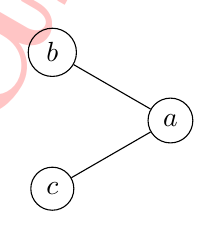
\begin{tikzpicture}[var/.style={circle,draw,minimum size=12pt}, node distance=1.5cm]
        \node[var] (a) at (0:1) {$a$};
        \node[var] (b) at (120:1) {$b$};
        \node[var] (c) at (240:1) {$c$};
        \draw (a) to (b);
        \draw (a) to (c);
    \end{tikzpicture}
    \caption{表 \ref{tab:活性分析} 对应的干扰图}\label{fig:干扰图}
\end{figure}

\subsection{代码优化}
本节内容仅供了解。

代码优化相比前面的内容略具「玄学」性,且不存在完美优化。编译界流传着「编译器从业者永不失业定理」,指的是编译器优化是一个复杂且困难的过程,尽管编译器可以执行多种优化操作,但这些优化操作的正确性和效果很难保证,因此编译器从业者的工作永远不会变得多余。‌

常见的优化方式:
\begin{itemize}[itemsep=0pt,parsep=0pt,leftmargin=1.5cm]
  \item 常量折叠:在编译器就计算表达式的值(可能用于语法制导翻译)
  \item 代数化简:利用某些代数运算的性质化简语句
  \item 死代码删除:静态移除程序中不可执行的代码
  \item 常量传播:配合到达定义分析实现,将变量唯一到达的定义传播到使用处
  \item 拷贝传播:类似常量传播,只不过将常量换为另一个变量
\end{itemize}

\backgroundsetup{contents=\includegraphics{下半示例.png}, center, scale=1, angle=0, opacity=1}
\BgThispage
\end{document} 